\documentclass[a4paper,12pt]{article}

\usepackage[a4paper, left=3cm, right=2cm, top=2cm, bottom=2cm]{geometry}
\usepackage[english]{babel} % language package.
\usepackage[utf8]{inputenc} % special characters, e.g. ü.
% \usepackage[T1]{fontenc} % font encoding.
\usepackage{microtype} % avoid Overfull \hbox warning.
\usepackage{float, graphicx}
\usepackage{booktabs} % needed for tables from pandas, using .to_latex.
\usepackage[table]{xcolor} % grey table rows.
\usepackage[flushleft]{threeparttable}
% \usepackage{tabular*}
\usepackage{subcaption}
\usepackage{caption}
\usepackage{amsfonts, amsthm, amssymb, amsmath} % serious mathematical typesetting.
\usepackage[onehalfspacing]{setspace} % Adapt line spacing.
\DeclareRobustCommand{\tbs}{\textbackslash} % used to display econsa\dev in bibliography.
\usepackage[backend=biber,
natbib=true, % command \citep originates from natbib.
style=authoryear, % reference style.
giveninits=true,
maxcitenames=2,
bibencoding=utf8,
uniquename=false]{biblatex}
\setlength\bibitemsep{\baselineskip} % increase space between entries in bibliography.
\addbibresource{bibliography.bib}
\usepackage[hidelinks]{hyperref} % hidelinks removes coloured boxes.
\usepackage{bookmark} % needed to run LaTeX only once for hyperref to create the references (call after calling hyperref).
\usepackage[noabbrev, capitalise]{cleveref} % load cleveref after hyperref.

\widowpenalty=10000 % page break (no single line hanging).
\clubpenalty=10000 % page break (no single line hanging).

% Custom commands.
\newtheorem{definition}{Definition}

\begin{document}

\begin{titlepage}

    \begin{center}

    \vspace*{1.0cm}

    {\LARGE
    \bfseries Assessing the Predictive Validity of Qualitative Sensitivity Measures \\
    \vspace*{0.5cm}
    % Untertitel
    }\\


    {\large
    \vspace*{4.0cm}
    Master Thesis Presented to the\\
    \vspace*{0.25cm}
    Department of Economics at the\\
    \vspace*{0.25cm}
    Rheinische Friedrich-Wilhelms-Universität Bonn\\

    \vspace*{2.0cm}
    in Partial Fulfillment of the Requirements for the Degree of\\
    \vspace*{0.25cm}
    Master of Science (M.Sc.)\\

    \vspace*{4.0cm}
    Supervisor: Prof. Dr. Philipp Eisenhauer\\

    \vspace*{2.0cm}
    Submitted in May 2021 by:\\
    Benedikt Heinrich Müller\\
    Matriculation Number: xxxxxx
    }

    \end{center}

    \end{titlepage}
\newpage

\tableofcontents
\newpage

\setcounter{page}{1}
\pagenumbering{Roman}

% Main body.

\setcounter{page}{1}
\pagenumbering{arabic}

\section{Introduction} \label{intro}

Economics is thinking in models that abstract from the actually existing economic systems by imposing assumptions on economic relations. Those assumptions are defendable as long as they are sufficiently realistic for the research question at hand \citep{F66}, what prompts the question, what sufficiently realistic means. Often, assumptions are decided upon by mathematical convenience: do the assumptions grant that the model is solvable, i.e. whether a solution exists in closed form and whether this solution is unique.

Due to the advancements in computational tractability we are less coerced to impose insufficiently realistic assumptions if numerical methods can be applied. That is, since even if the model at hand does not have an analytical solution, one can still obtain an approximate solution by applying numerical methods \citep{MF04}.

[Example with Rust model and why no analytical solution exists.]

\noindent Consider the following model
\begin{equation*}
Y = f(X),
\end{equation*}

where $Y$ is the response variable that depends on the values of some independent variables $X$. Let $X$ denote the vector $X = (X_1, \dots, X_k)' \in \mathbb{R}^k$, where $k$ is the number of independent variables. Let $x$ be the vector of specific values assigned to $X$, i.e. one realisation of $X$. Let $f(\cdot)$ denote a function that describes in which way $Y$ depends on $X$. This function may be some complex function (e.g. computer code) or a model that can be solved by numerical methods only. Thus, $f$ is generally not available in closed form and, hence, the relationship between $Y$ and $X$ is considered a black box.

In the remainder of this work, I name $Y$ the (model) output and the vector $X$ the (model) inputs. In this work I will consider $X$ as being stochastic, that is, the $X_i$, $i = 1,\dots, k$, follow a joint cumulative distribution function $G(X)$. Thus, although $f$ is assumed to be a deterministic function of $X$, the output $Y$ is also stochastic due to the uncertainty in $X$ \citep{SNS16}. Sensitivity analysis sheds light on this input-output relationship \citep{BP16}.

In the context of structural econometrics sensitivity analysis has an important role. Structural econometrics imposes structure on the relationship between economic parameters \citep{LM17}. The structural model is then taken to the data and deep economic parameters are estimated \citep{LM17}. Structural econometrics can be used to investigate counterfactual policies by quantifying the effects of a policy on some output \citep{LM17}. If these models are actually used for policy making, the structural model and its assumptions have real-world consequences. The question arises whether the imposed model assumptions are realistic enough to inform policy. Therefore, thorough modelling is crucial for structural econometrics.

Sensitivity analysis analyses how sensitive the model outcome is to model inputs \citep{R21}. Any assumption we impose can be such an input \citep{R21}. For example, an estimated parameter we assume to be deterministic by assigning a value to it, we implicitly neglect that the estimate is subject to uncertainty \citep{R21}. Making this assumption can be problematic if the model output is very sensitive to the value assigned to this input. Such an input we call ``important". Sensitivity analysis can guide research by identifying these important inputs \citep{R21}. For example, we could put more effort into estimating such important inputs more precisely, thus reducing output uncertainty.

In order to understand the model behaviour, sensitivity analysis is a way of learning about the input-output relationship of the model at hand \citep{BP16}. One can generally structure sensitivity analysis into local and global methods of sensitivity analysis \citep{BP16}. Local methods conduct sensitivity analysis around a certain point, or base case, $x_0$, in a deterministic framework, i.e. no probability distribution is assigned to $X$ \citep{BP16}. In contrast, when performing global sensitivity analysis, we find ourselves in a stochastic context, which requires knowledge of the distribution of $X$, be it joint or marginal with or without dependence between the inputs \citep{ST02}. The settings for which sensitivity analysis methods can yield useful information are further discussed in \cref{var_based_sa}.

The result of performing sensitivity analysis is some sensitivity measure, that depends on the sensitivity analysis method we apply to the context we find ourselves in. In this work, I assess the predictive validity of Morris indices, a qualitative sensitivity method \citep{M91}. Qualitative sensitivity methods aim at i. identifying uninfluential inputs and ii. ranking inputs with respect to their importance \citep{BP16}. I compare the performance of the Morris method for dependent inputs as proposed by \citet{GM17} to Shapley effects, a variance-based quantitative sensitivity method \citep{O14}.

Variance-based sensitivity analysis, a method that evaluates the importance of an input by assigning to it the expected reduction in output variance if this input was known with certainty \citep{BP16}. Shapley values are a concept from game theory introduced by \citet{S53}. The main advantages of Shapley values for sensitivity analysis are that they are as easily applied to dependent inputs as they are interpreted. Furthermore, Shapley values satisfy a range of desirable properties, the most important being efficiency and the null-player property \citet{S53, O14}. In the context of sensitivity analysis, \citet{SNS16} use the term Shapley effects. Despite of these appealing features, estimation of Shapley effects can be computationally demanding \citep{SNS16}.

This is where the Morris method comes into play, since it promises to serve similar purposes as Shapley effects, but come at a lower computational cost. In this work I estimate Morris indices for a classical structural econometric model, the single-agent dynamic stochastic model of discrete choice introduced by \citet{R87} and compare these to Shapley effects. Interestingly, I find that the Morris method is a worthy substitute for Shapley effects since they perform very well in identifying uninfluential inputs and in ranking the inputs accordingly for the Rust model.

% One set of common variance-based sensitivity measure are the total and first-order effects, or Sobol' indices, introduced by \citet{S93} for independently distributed input variables, which are based on an Analysis of Variances (henceforth ANOVA) decomposition. One obvious drawback of the Sobol' indices in the original definition is that they rely on the assumption of inputs independence. Even if the ANOVA decomposition is adapted to handle dependent inputs, they suffer from problems \citep{OP17} which are discussed in \cref{var_based_sa}. \citet{OP17} suggest using Shapley values instead, which were suggested in the context

\section{The Rust Model} \label{rust_model}

This section sets up the model whose input-output relationship I want to shed light on. I consider the single-agent dynamic discrete choice model of \citet{R87}.

\subsection{Bus-Engine Replacement Model}

Every period an agent needs to decide whether to replace the engine of a bus in the carpark or to conduct standard maintenance operations. The Rust model assumes optimal behaviour of the agent and asks what the implied deep economic parameters are, given this optimal behaviour.

The model output I consider is implied annual demand for engine replacements. Model inputs are engine replacement costs and a cost parameter that is part of the agent’s utility function. In the Rust model these variables are estimated but I consider them as inputs for the computation of implied annual demand. Since the inputs are estimated, they are subject to uncertainty. It is the influence of the inputs on the output I want to analyse. Applying sensitivity methods requires the simulation of the input variables. To that end, information about the distribution of the inputs is needed. The variance-covariance matrix of the inputs is estimated in \cref{model_setup} % especially for calculating the variance-covariance matrix and mean vector of the inputs.

In \citet{R87} an agent needs to manage a pool of buses for public transportation. Each period a bus exhibits an observable accumulated mileage state (odometer state) $x$ and other state variables $\varepsilon$, that are unobserved by the econometrician. The agent has to decide whether to perform standard maintenance or an expensive engine replacement. The agent’s decision in period $t$ is
\begin{equation*}
i_t\ =
\begin{cases}
0,\ \text{standard maintenance}, \\
1,\ \text{replace engine}.
\end{cases}
\end{equation*}

\noindent If replacement is chosen, the accumulated mileage state $x$ is set to zero. Otherwise, the bus is used for another period with standard maintenance and $x$ increases until the next period. Note that $x$ needs to be discretised for estimation purposes. I follow \citet{R87} and discretise the state space into 175 grids with a size of each bin of $2\,571$ miles.

The agent’s utility function given state $(x, \varepsilon)$ is described by
\begin{equation}
u(x, i, \varepsilon; \theta_1, RC)=v(x, i; \theta_1, RC)+\varepsilon(i), \label{utility}
\end{equation}

where
\begin{equation*}
v(x, i; \theta_1, RC)=
\begin{cases}
-c(x; \theta_1), & \text{if}\ i=0,\\
-RC-c(0;\theta_1), & \text{if}\ i=1,
\end{cases}
\end{equation*}

\noindent and $\varepsilon(i)$ denotes utility shocks. In the above expression, $RC$ represents the expected costs of an engine replacement, that is, net the possible payoff of selling the old engine. $c(x; \theta_1)$ is a cost function of operating a bus at state $x$. $\theta_1$ is a vector of structural parameters. I consider the linear cost function $c(x; \theta_{11}) = 0.001 \theta_{11} x$.
\cref{utility} reflects the trade-off between minimising maintenance costs and minimising unexpected, costly engine failures, e.g. due to loss of customer's goodwill.

How the state $(x, \varepsilon)$ changes over time, depends on the choice $i_t$ and is described by the Markovian transition density $p(x_{t+1}, \varepsilon_{t+1} \mid x_t, \varepsilon_t, i_t; \theta_2, \theta_3)$, where $\theta_2$ is assumed to be Euler’s constant and $\theta_3$ is a vector of transition probabilities. Markovian means that $p$ depends on $ (x_t, \varepsilon_t) $ only and not on other past states.

The discount factor is denoted $\beta \in (0,1) $. Given state $ (x_t, \varepsilon_t) $, the agent, choosing a sequence of decisions, maximises
\begin{equation*}
\max_{\{i_t, i_{t+1}, i_{t+2}, \dots\}}  \mathrm{E} \left[\sum_{\tau=1}^\infty \beta^{\tau-t} u(x_{\tau}, i_{\tau}, \varepsilon_{\tau}; \theta_1, RC) \right].
\end{equation*}

By $p$ being Markovian, the optimal decision is time-invariant. Thus, drop time indices. The decision problem is now defined by the solution to the Bellman equation
\begin{equation*}
	V(x, \varepsilon)=\max_i \{ v(x, i; \theta_1, RC)+\varepsilon(i) + \beta \int_{x'} \int_{\varepsilon'} V(x', \varepsilon')p(x', \varepsilon' \mid x, \varepsilon, i; \theta_2, \theta_3)dx' d \varepsilon' \}.
\end{equation*}
% \begin{multline*}
% V(x, \varepsilon)=\max_i \{ v(x, i; \theta_1, RC)+\varepsilon(i) + \\
% \beta \int_{x'} \int_{\varepsilon'} V(x', \varepsilon')p(x', \varepsilon' \mid x, \varepsilon, i; \theta_2, \theta_3)dx' d \varepsilon' \}.
% \end{multline*}

The above problem is simplified by imposing some further assumptions to ease the estimation process. The model is solved by using the so called Nested Fixed Point algorithm \citep{R87}. The parameters to be estimated are combined in a vector $\theta=(\theta_3, RC, \theta_{11}) $. The estimation procedure via Maximum Likelihood is conducted by first estimating the transition probabilities $\theta_3$. In a second step, the parameters $RC$ and $\theta_{11}$ are estimated.\footnote{I do not go into further details of how this model is solved. For details see \citet{R87}.}

\subsection{Distribution of the Input Variables} \label{model_setup}

The Maximum Likelihood estimator is asymptotically normally distributed \citep{R73}. Thus, I estimate the variance-covariance matrix of $\theta_{11}$ and $RC$ by a Monte Carlo simulation. Note that this general setup is used in \cref{comp_shap} and \cref{comp_morris} as well. For solving the model, I use the simulation and estimation capabilities of the Python \textit{ruspy} package \citep{OSE19}.\footnote{I chose \textit{scipy\_L-BFGS-B} as the solver for the Nested Fixed Point algorithm \citep{SP20}.} The estimation of the variance-covariance matrix is conducted in three steps.

Firstly, I set the true parameters in $\theta$. I chose to consider three transition probabilities, i.e. the mileage state $x$ can increase from the current period to the next by two grids at most. I set
\begin{align*}
\theta_3 &= (\theta_{30}, \theta_{31}, \theta_{32})=(0.39189182,\ 0.59529371,\ 0.01281447),\\
RC &= 10.07780762,\\
\theta_{11} &= 2.29417622.
\end{align*}

\noindent Note that $RC$ is scaled by $0.001$ for estimation purposes. I consider a total of 50 buses for 120 periods (months, i.e. in total ten years).

\begin{table}
	\centering
	\caption{Variance-Covariance Matrix of the Input Variables}
	\label{cov}
	\begin{threeparttable}
	\centering
	\begin{tabular}{lrr}
\toprule
{} &      $RC$ &  $\theta_{11}$ \\
\midrule
$RC$          &  1.604736 &       0.605903 \\
$\theta_{11}$ &  0.605903 &       0.273094 \\
\bottomrule
\end{tabular}

	\begin{tablenotes}
	\small
	\item \textit{Notes:} Estimation based on $10\,000$ data sets.
	\end{tablenotes}
	\end{threeparttable}
\end{table}

Secondly, I simulate $10\,000$ data sets from the above true parameters and estimate $\hat{\theta}, \hat{\theta}$ being the vector of estimated structural parameters.

Thirdly, from the $10\,000$ parameter estimates of the replacement costs $\widehat{RC}$ and the slope parameter of the cost function ${\hat{\theta}}_{11}$, I calculate the sample variance-covariance matrix which is shown in \Cref{cov}. \Cref{cov} and \cref{correlation} show that $\widehat{RC}$ and ${\hat{\theta}}_{11}$ correlate, hinting that inputs in the Rust model are indeed dependent.

\subsection{Derivation of Implied Annual Demand}

\begin{figure}[t]
	\caption{Correlation Between the Input Variables}
    \label{correlation}
	\centering
	\vspace*{-4mm}
	\begin{centering}
	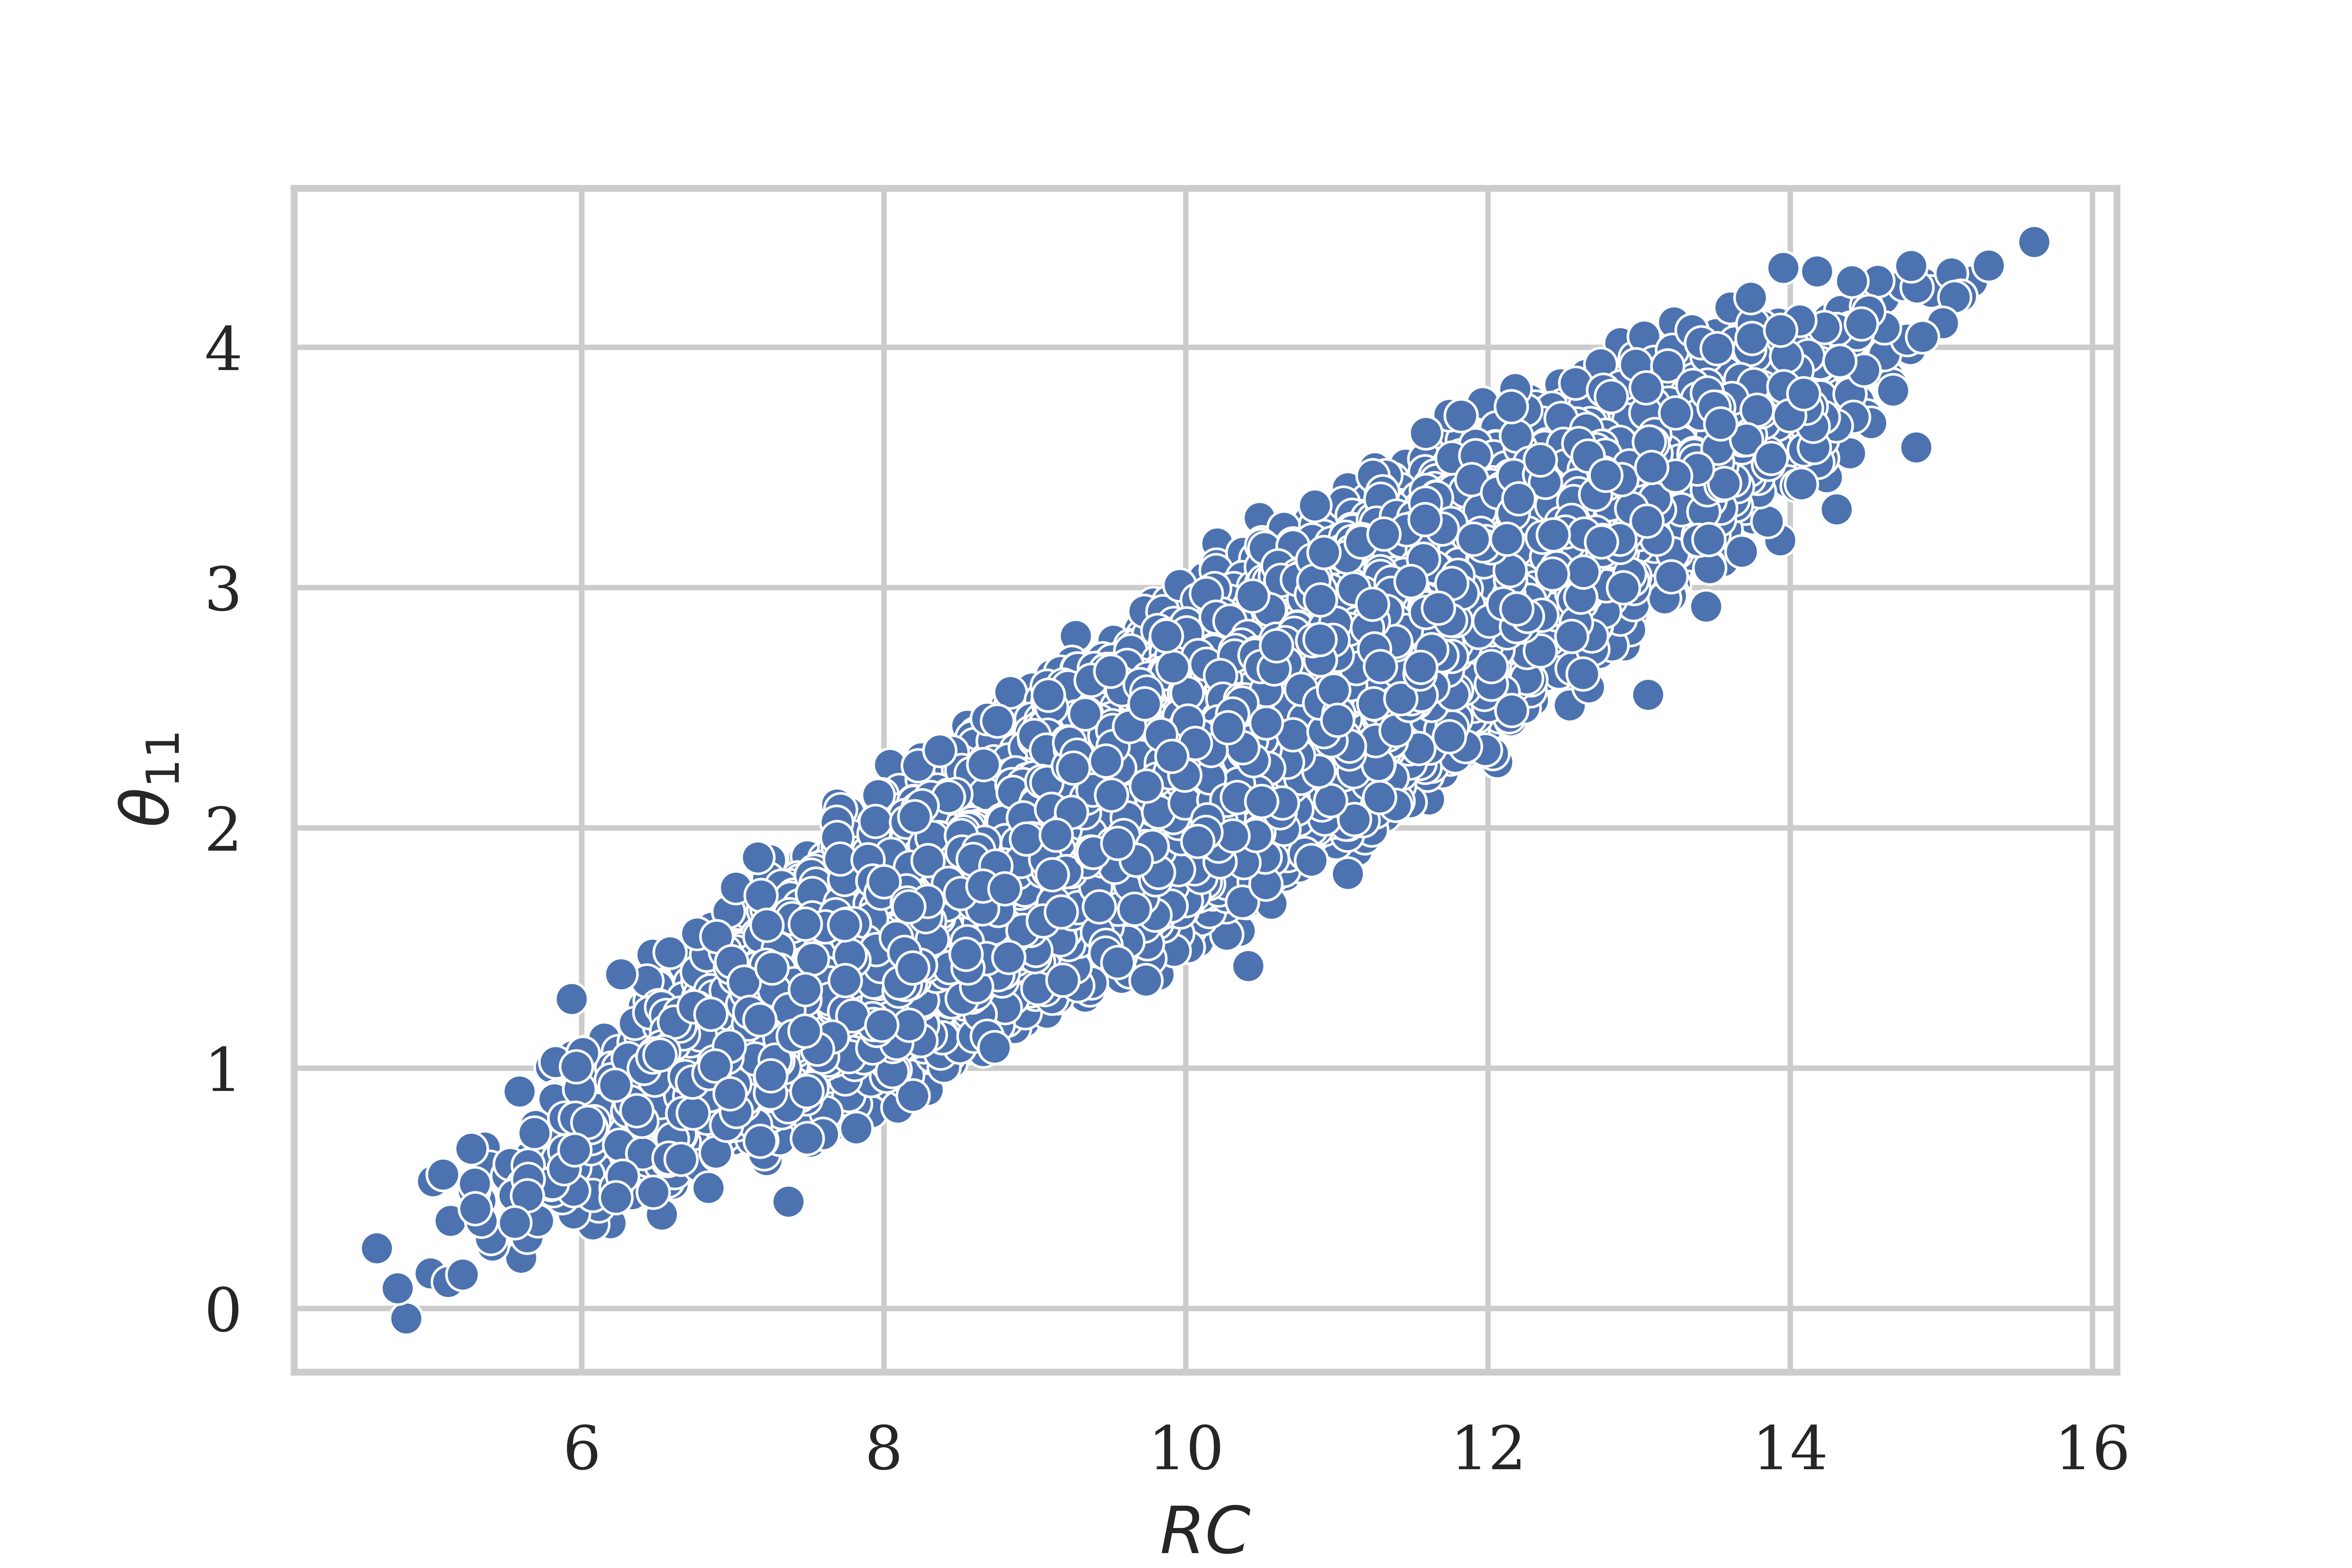
\includegraphics[scale=0.9]{../figures/correlation_rc_theta.png}
	\end{centering}

	\small
	\textit{Notes:} $10\,000$ estimated values of $RC$ and $\theta_{11}$.

\end{figure}

\citet{R87} shows how we can derive further quantities from the parameter estimates. He derives the implied annual demand (henceforth, demand) for bus-engine replacements, which is computed by
\begin{equation*}
\tilde{d}(RC)=\sum_{t=1}^{12} \sum_{i=1}^{M} {\tilde{i}}_t^m,
\end{equation*}

\noindent where $M$ is the number of buses and ${\tilde{i}}_t^m$ is a realisation of the process $(i_t^m, x_t^m)$, with $m$ being the bus index. Here, $M=50$. Since we consider the \textit{annual} demand, we sum over twelve months. Recall that a period is represented by one month, so we end up with the annual demand for 50 buses. $\tilde{d}(RC)$ is stochastic, since ${\tilde{i}}_t^m$ is. Let $\pi_m(x_0^m, i_0^m)$ denote the distribution of the initial state for each bus $m$. Given this, we can compute the probability distribution of $\tilde{d}(RC) $ by the transition probability $P(i_t \mid x_t, \theta)p(x_t \mid x_{t-1}, i_{t-1}, \theta_3) $. Note that $P(\cdot)$ depends on $\theta$, i.e. it depends on $RC$ as well. We can compute demand for a range of values for $RC$. In my analysis I compute demand for a single value of $RC$ only, which is arbitrarily set to $RC^{demand}=11.5$, i.e. $11\,500$ money units. \citet{R87} considers the expected demand, i.e. $d(RC)=E[\tilde{d}(RC)]$. Assuming that the initial state distribution $\pi$ is the long-run equilibrium distribution of $(i_t, x_t)$, $\pi$ is the solution to
\begin{equation*}
\pi(x, i)=\int_y \int_j P(i \mid x, \theta) p(x \mid y, j, \theta_3) \pi(dy, dj).
\end{equation*}

Note, that $\pi$ is a function of $\theta$. Assuming further that the processes $ (i_t^m, x_t^m)$ and $(i_t^k, x_t^k)$ are independent for $k \neq m$, i.e. the process of a bus is independent from the process of any other bus, we can write
\begin{equation*}
d(RC)=12 \cdot M \cdot \int_0^{\infty} \pi(dx, 1).
\end{equation*}

To see how the uncertainty in the inputs $(RC, \theta_{11})$ propagate to the output, demand, see \cref{uncertainty}. I again use \textit{ruspy} for the computation of the demand at $RC^{demand}$. I compute demand for $100\,000$ simulated data sets. The output is normally distributed as can be seen in \cref{uncertainty} with mean 58.67 and variance 41.83. Sensitivity analysis can identify the inputs that are responsible for this large variability in the model output.

Now, that the model, i.e. how the output depends on the inputs, has been clarified, we are ready to consider the sensitivity methods applied in this thesis.

\begin{figure}[t]
	\caption{Uncertainty Propagation}
    % \floatfoot{A note}
    \label{uncertainty}
	\begin{centering}
	\vspace*{-4mm}
	\begin{centering}
		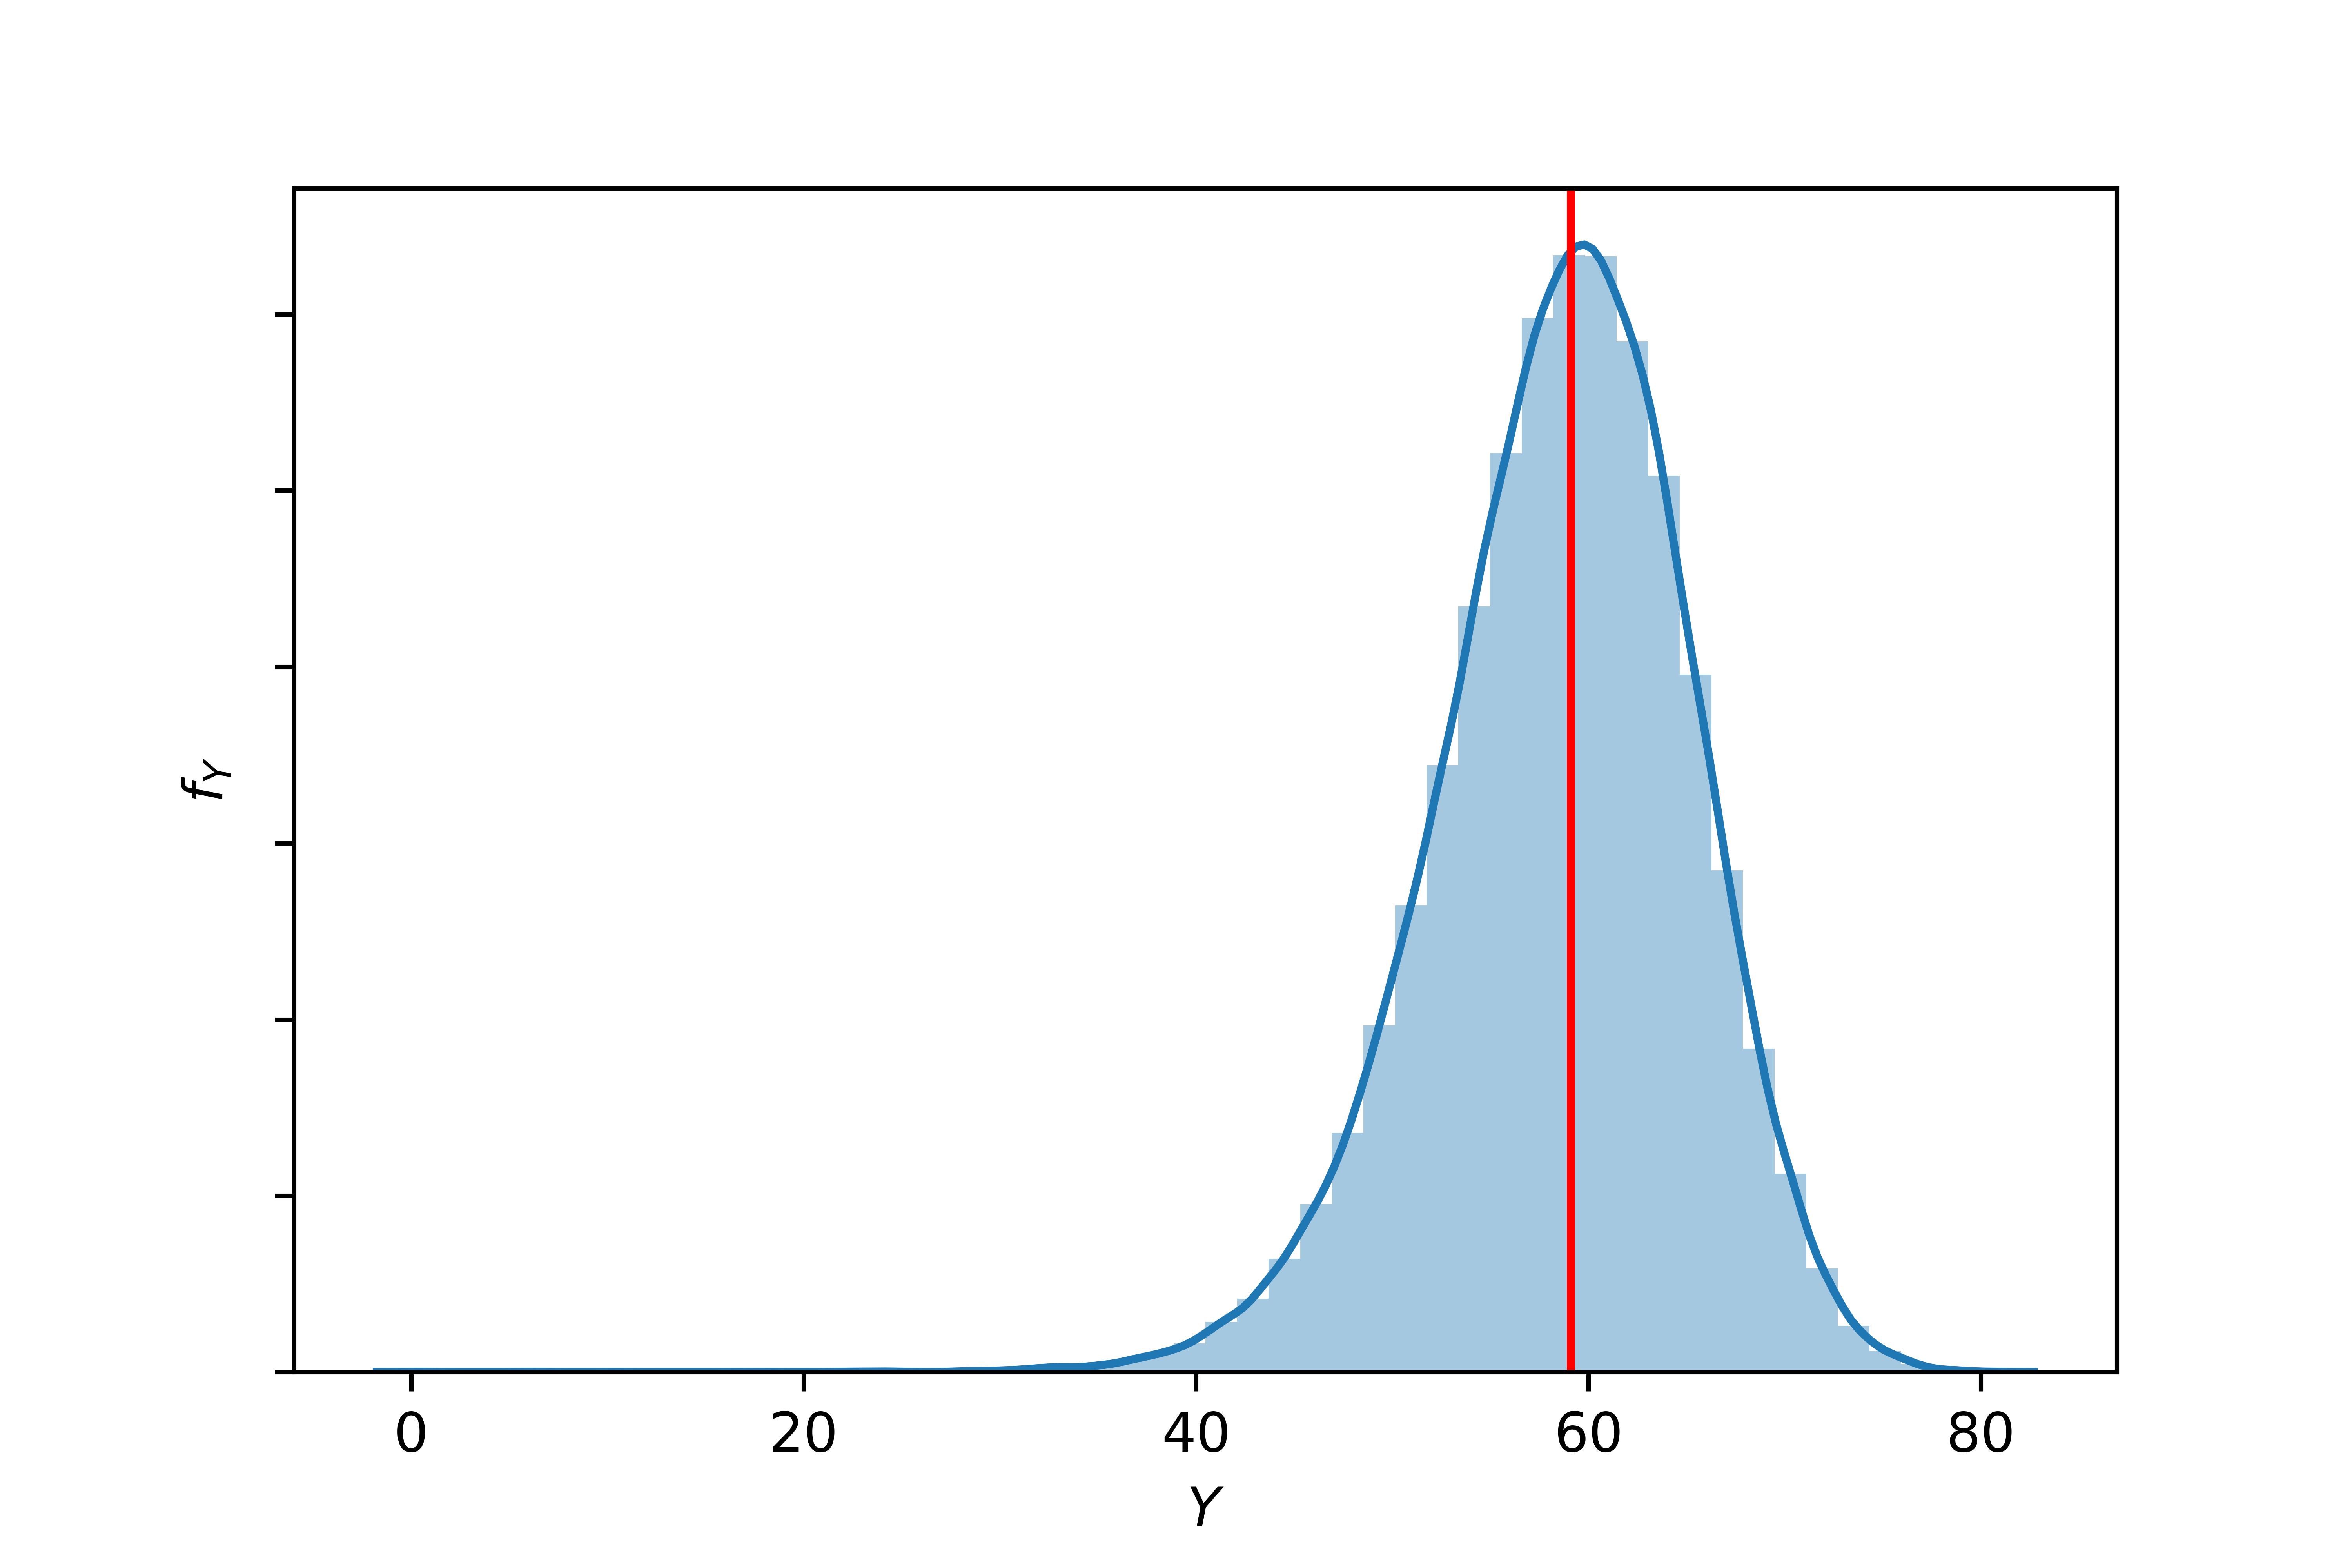
\includegraphics[scale=0.9]{../figures/uncertainty_propagation_100000.png}
	\end{centering}
	\end{centering}

	\small
	\textit{Notes:} Estimated implied annual demand for $100\,000$ simulated data sets. The horizontal line shows the implied annual demand at the \textit{true} parameter values $(RC, \theta_{11})$. This \textit{true} demand amounts to $59.09$.
\end{figure}

\section{The Benchmark: Computation of Shapley Effects} \label{comp_shap}

This section introduces Shapley effects for sa. Shapley effects will serve as a benchmark for evaluating the performance of the sm derived by the Morris method.

\subsection{Shapley Values in Economics}

The Shapley value is a concept from cooperative game theory, introduced by \citet{S53}. It is a value that informs about how to fairly distribute the profit of a product that was created by a team effort. Fairly here means, that any player receives as much of the gain as he or she contributed to the team effort. As individual contributions are not directly observed, \citet{S53} proposes the following value. The Shapley value ensures that every individual receives at least as much as if he or she had if acted independently \citep{IP19}.

Consider a game with $k$ players, where $K$ denotes the set of all players, the grand coalition. A coalition is a subset $J \subset K$. Let $- J$ denote the complement set of $J$, i.e. $- J = K \setminus{J}$. The corresponding game is defined by a coalition value function that maps each coalition $J$ to the value attained by this coalition, i.e. $val: 2^K \to \mathbb{R}_{\geq 0}$, where $2^K$ denotes the power set of $K$ (set of all subsets of $K$) \citep{SNS16}. It is generally assumed that $val(\emptyset) = 0$. The following definition is strongly inspired by the one found in \citet{PRB20}:

\begin{definition}

Given a coalition worth function $val$, the marginal contribution of player $i$ joining coalition $J$ is $mar(J,\ i)=val(J \cup \{i\}) - val(J)$. The Shapley value is then defined by
\begin{equation}
\begin{split}
\phi_{i} (val)& = \sum_{J \mid i \notin J} \frac{\vert J \vert ! (k - \vert J \vert - 1) ! }{ k !} (val(J \cup \{i\}) - val(J)) \\
& = \frac{1}{k} \sum_{J \mid i \notin J} \binom{k-1}{\vert J \vert}^{-1} mar(J,\ i).
\end{split}
\end{equation}

\end{definition}

In words, one considers every coalition of players and evaluates by how much the inclusion of player $i$ increases the overall profit of the coalition. This is achieved by subtracting the value generated by the members of coalition $J$ from the value created by the larger coalition that includes coalition $J$ and player $i$. In the context of a game, the marginal value for each coalition is divided among all members of this coalition, e.g. if the coalition has one member only, the entire marginal value is gained by this player. One can also interpret the Shapley value as the expected payoff from joining a coalition or from leaving the complementary coalition \citep{PRB20}.

\citet{S53} shows that $\phi_i$ satisfies the following four axioms and that the Shapley value is the only value that satisfies all four axioms at the same time. Note that Shapley values normalised by total profit are considered.

\begin{itemize}
    \item Pareto efficiency: $\sum_{i=1}^{k}\phi_i=1$.
	\item Symmetry: If $val(J \cup {i})=val(J \cup {j})\ \forall\ J \subseteq K \setminus{\{i,\ j\}}$, then $\phi_i = \phi_j$.
	\item Linearity: $\phi_i(val_1 + val_2)=\phi_i(val_1)+\phi_i(val_2)$.
	\item Null-player: If $\forall J,\ mar(J,\ i) = 0$ holds then $\phi_i(val) = 0$.
\end{itemize}

Pareto efficiency assures that nothing of the profit gained by the team is wasted. Normalised by the total profit, the Shapley value gives the share attained by each individual in the game. Symmetry results into all players who contributed the same to the common product, receiving the same payoff, reflecting the meritocratic principle. The null-player axiom ensures that players that do not contribute to the team effort at all, do not receive any share in the profits. Especially axioms 1 and 4 are desirable in the context of the Shapley value as a variance-based sm.

\subsection{Variance-based Sensitivity Analysis} \label{var_based_sa}

There are several purposes for which one can apply sa methods in general. Note, that in sa one refers to input variables by the term factors \citep{R21}. In their textbook, \citet{STC04} summarise the following four possible objectives of sa.

Factors Prioritisation (FP): In the FP setting, one determines on which inputs applied, uncertainty reduction results into the largest reduction in output uncertainty. SA determines the importance of an input variable. Applied to all inputs, one can derive a ranking of all inputs in order of importance. FP can guide research by prioritising inputs. Inputs are identified for which better experimental measurement can reduce output uncertainty the most, supposing that additional information costs the same for alle inputs.

Factors Fixing (FF): The FF setting allows one to determine the least influential inputs. These then can be fixed at a specific value without losing information in the model output. FF can also be seen as inputs screening. One would want to fix the least influential inputs to reduce dimensionality of the model and thus the complexity and computational burden.

Variance Cutting (VC): VC informs about which inputs to fix to arrive at a certain desired value of the output variance, under the condition that the smallest number of inputs are fixed. VC is most useful for risk assessment.

Factors Mapping (FM): If one cares about the input importance in certain regions of output values only, one can apply FM. First, one classifies output values into groups and only then employs the importance exercise. So, the inputs are determined that contribute the most to producing output values in a target region. E.g. one could be interested in a certain percentile of the output range. The term mapping stems from mapping the importance of the inputs to the categories of $Y$.

SA does address more fundamental objectives of mathematical modelling and the analysis of systems that can be achieved directly from the above settings and are summarised in \citet{R21}. By sa, one can achieve or conduct a. scientific discovery, i.e. identification of causal relationships, b. dimensionality reduction, i.e. determination of the least important inputs, which is achieved by FF, c. data worth assessment, which relates to FP, and d. decision support \citep{R21}.

In global sa, where, as one may recall, inputs are probabilistic in nature, one distinguishes six classes of sa methods \citep{BP16}. The sensitivity indices discussed and applied in this work belong to the area of variance-based sensitivity measures. Variance-based sensitivity measures are obtained by determining the expected reduction in output variance due to knowing input i with certainty \citep{BP16}. These methods are based on the classical formula for the law of total variance
\begin{equation}
V[Y]= V[E[Y \mid X_J]] + E[V[Y \mid X_J]]
\end{equation}

\noindent assuming that $f(X) < \infty$, where the $V$ operator stands for the unconditional variance of $Y, V[\cdot \mid \cdot]$ for the conditional variance, and $E[\cdot \mid \cdot]$ denotes the conditional expectation. The above expression decomposes total variance into the explained and the unexplained component (citep!).

A variance-based sensitivity measure determines much output variance is attributable to each input $i$ \citep{BP16}. Variance-based global sa is not applicable to decision variables, since global sa attaches a distribution to input variables, implying that inputs are uncertain \citep{SNS16}. Recall that due to this uncertainty in the inputs $X_K$ the output $Y$ is uncertain as well. $V[Y]$ measures this uncertainty in the output, where $V[Y]$ is taken according to the joint distribution of $G_K$. In the variance of the model output, there are three parts of variances; the one caused by every input in isolation, the one that is caused by interaction effects among inputs, and one that is due to input dependence.

\citet{S93} introduced often used variance-based sensitivity indices that attribute the variance reduction to each subset $J \subset K$ using an ANOVA decomposition. To ensure uniqueness of the ANOVA decomposition employed by \citet{S53}, one needs to assume independence of model inputs \citep{GM17}. Sobol' indices were introduced as a subset importance measure \citep{SNS16}. For the purposes of sa we let the subsets be the single inputs, i.e. the subsets under considerations are singletons. The Sobol' indices are then defined as
\begin{align}
S_i &= V[Y]^{-1} V[E[Y \mid X_i]]\\
S_i^T &= V[Y]^{-1}(V[Y] - V[E[Y \mid {X_{- i}}]])
\label[equation]{total_sobol}
\end{align}

\noindent where $X_{- i}$ is the subset of input variables without input $i$. What follows does apply to models with independent inputs only. The sensitivity measure $S_i$ is called the first-order sensitivity index. $S_i$ represents the share of output variance reduced by the isolated effect of input $i$, excluding contributions in variance reduction by interactions between input $i$ and the remaining $(K-1)$ inputs. The subtrahend in the nominator of \cref{total_sobol} can be seen as the expected variance reduction when $X_i$ is fixed at a certain value, i.e. if we know $X_i$ with certainty \citep{SNS16}. $S_i^T$ is called the total sensitivity index. $S_i^T$ complements $S_i$ in the sense that it measures the total effect of $X_i$ in the output variance, including interaction effects \citep{SNS16}. It can be considered the expected remaining output variance, when all values of the inputs are known, except for the value attached to $X_i$ \citep{SNS16}. By normalising both measures by $V[Y]$, it is clear that the value s of $S_i$ and $S_i^T$ are in the interval $[0, 1]$, since the numerators in equations xy and yz are always smaller than the total variance \citep{GM17}. For the relationship between $S_i$ and $S_i^T$ the weak inequality $S_i\ \le\ S_i^T$ holds true, while equality only holds when there are no interaction effects between $X_i$ and $X_{- i}$. Note that the terms indices and effects are used interchangeably.

Under input independence, the Sobol' indices have a clear interpretation. If $S_i$ is large, then the corresponding input $X_i$ is an influential input with respect to the output variance reduction \citep{GM17}. In contrast, a small first-order effect $S_i$ does not imply that $X_i$ is an uninfluential input, if strong interaction effects are present \citep{GM17}. As $S_i^T$ measures the total variance contribution by $X_i$, one can infer from a small $S_i^T$ that $X_i$ is indeed not uninfluential \citep{GM17}. If so, $X_i$ could be fixed at a certain value without causing changes in the model output variance \citep{GM17}.

Evaluating $S_i$ and $S_i^T$ one can also learn something about the structure of the model one is analysing, always assuming that inputs are independent. The model structure can be determined by the sums $\sum_{i \in K} S_i$ and $\sum_{i \in K} S_i^T$ \citep{GM17}.If both sums are equal to one, interaction effects are negligible , since the model is additive in nature. The model is non-additive if $\sum_{i \in K} S_i < 1$ and $\sum_{i \in K} S_i^T > 1$ \citep{GM17}. Thus, it can be inferred that interaction effects cannot be ignored and play a role in the system under consideration.

Recall that the statements about the model structure and input importance do not hold if inputs are dependent. In the case of dependence, one cannot simply apply the ANOVA decomposition since it is no longer unique \citep{O14}. In the Rust model, there are two input variables, $RC$ and $\theta_{11}$. As one can see in \cref{model_setup}, there exists significant dependence between the inputs. Thus, Sobol' indices should not be used. Another variance-based sensitivity measure are the now popular Shapley effects, which can be used also in the context of dependence. They are derived in the following section.

\subsection{Shapley Effects for Sensitivity Analysis}

In the context of sa, \citet{SNS16} named Shapley values Shapley effects, which were first suggested as a variance-based sensitivity measure by \citet{O14}. According to \citet{PRB20} the Shapley effect is becoming more and more popular in sa.

When applied as a sensitivity measure, the interpretation of the Shapley value changes. $X_i$ is now interpreted as a model input instead of a player in a game. A coalition is now a subset of model inputs. \citet{O14} defines the function $\widetilde{val}$ as a function that assigns the explanatory power of this subset of inputs to this subset. That is, the function $\widetilde{val}$ assigns the conditional variance to a subset of inputs, $\widetilde{val}(J)=V[Y]^{-1}V[E[Y \mid X_J]]$ and $\widetilde{val}$ measures the reduction in $V[Y]$ due to the inputs in $J$ \citep{SNS16}. \citep{SNS16} show that the following alternative formulation of the value function results into the same Shapley effect.
\begin{equation}
val(J)=E[V[Y \mid X_{- J}]]
\end{equation}

\noindent $val(J)$ can be interpreted as the remaining variance of $Y$, given the values of the inputs in $- J$ are known. Both formulations satisfy the following two requirements
\begin{align}
val(\emptyset)& = 0\\
val(K)& = V[Y].
\end{align}

\noindent In words, the value of the empty input subset should be zero and the value of the set of all inputs should equal the entire output variance. In this work I consider the value functions normalised by $val(K)=V[Y] $ to get Shapley effects normalised to the interval $ [0,\ 1] $. The most appealing properties of Shapley effects are that they satisfy the following two conditions (compare to axioms 1 and 4).
\begin{align}
\sum_{i=1}^{k}\phi_i& = 1\\
\phi_i& \geq 0,\ \forall \ i=1, ..., k.
\end{align}

\noindent So, the Shapley effects calculated for a model sum up to one and each Shapley effect is weakly larger than zero. Hence, the Shapley effects are input importance measures in terms of the expected output variance reduction induced by $X_i$. The non-negativity condition ensures that Shapley effects are always clearly interpretable. Note that due to the uncertainty in the computation process there exists the possibility of Shapley effects turning out to be below zero. By increasing sample sizes, this phenomenon should be mitigated.

Shapley effects can be used to compare input importance, that is, inputs can be ranked according to their contribution to output variance reduction. Furthermore, the differences between values of Shapley effects can be interpreted.

Recall the three parts of model output variance as discussed in \cref{var_based_sa}: variance due to the isolated effect of an input (i.e. the main variance), due to interaction effects, and due to dependence among inputs. Shapley effects take all three into account. In this regard they differ from first-order and total Sobol' indices as defined in \cref{var_based_sa} \citep{O14}.

In comparison to Shapley effects one has to acknowledge that Sobol' indices can inform about the model structure as discussed in \cref{var_based_sa}. In addition, Sobol' indices address more sa settings than Shapley effects, if inputs are independent. Shapley effects can be applied to FF only, since they distribute the effect of interactions between inputs equally across all inputs contained in the current subset \citep{IP19}. FP cannot be precisely conducted by using Shapley effects, since one cannot distinguish between contributions of main variance and variance contributions due to due to interactions \citep{IP19}.

Shapley effects yield a single value for each input that serves as the sensitivity measure, as opposed to Sobol' indices, which yield the first-order and total effects., i.e. two measures per input. Especially when computing sensitivity indices for studies that evaluate scientific phenomena, having a single value per input that informs about the variance contribution is very useful \citep{SNS16}. Furthermore, when this measure considers main and interaction effects and can also handle input dependence, one has a very useful and versatile sensitivity measure.

Sobol' indices for dependent inputs have been proposed \citep{MTA15}. This strategy is based on the estimation of four sensitivity indices, instead of the two measures in the case of input independence, elevating the practical usefulness of Shapley effects even more. In case of input dependence, Sobol' indices require a complicated ANOVA decomposition, whereas Shapley effects do not rely on such variance decompositions \citep{IP19}. When applying Shapley effects, one would not even need to know whether input dependence or independence prevails.

Several algorithms exist for estimating Shapley effects. See the following section.

\subsection{Algorithm} \label{comp_alg}

The algorithm for the computation of Shapley effects needs to allow for conditional sampling of dependent inputs. Otherwise, some of the advantages of Shapley effects cannot be exploited. I use algorithm 1 from \citet{SNS16}, see algorithm 1 in this paper.

Shapley effects consider all input subsets. To iterate over all subsets, \citet{SNS16} restate the equation for Shapley effects to iterate over all permutations of model inputs. For instance, let $k=5$. Then, $K=\{1,\ 2,\ 3,\ 4,\ 5\}$. There exist $5!$ permutations, where one is $\pi'=(2,\ 4,\ 3,\ 5,\ 1)$. Let the set of all permutations of $K$ be denoted by $\Pi(K)$. Further, let $P_i(\pi)$ denote all inputs in permutation $\pi$, that come before input $i$. In the above example, if $i=3$, then $P_3(\pi')=\{2,\ 4\}$. Using the permutation representation, \citet{SNS16} state the marginal contribution due to input $i$ as $val(P_i(\pi) \cup\{i\}) - val(P_i(\pi))$. By considering all permutations of $K$, we can restate the equation for the Shapley effects for input $i$ as
\begin{equation}
\phi_i=\sum_{\pi \in \Pi(K)} (k!)^{-1} (val(P_i(\pi) \cup\{i\}) - val(P_i(\pi))).
\end{equation}

The algorithm of \citet{SNS16} exploits the fact that their permutation-based algorithm evades redundant model evaluations by going through the permutations beginning with the smallest subset. The contribution of the preceding subset is subtracted from the contribution of the current subset. The marginal contribution is then computed by writing
\begin{equation}
val(P_{\pi(j)}(\pi) \cup \{\pi(j)\}) - val(P_{\pi(j)}(\pi)),
\end{equation}

\noindent where $\pi(j)$ denotes the input at position $j$ in permutation $\pi$. In the above permutation $\pi'$, at position 2 we have input 4, i.e. $\pi'(2)=4$.

To see for which subsets the algorithm performs evaluations of $val$, consider the below example. For instance, following \citet{SNS16}, if $k=3$ and $\pi=(1, 3, 2)$, the algorithm computes
\begin{align*}
\Delta_1 &=val(\{1\})-val(\emptyset),\ set\ prevC=0, \\
\Delta_2 &=val(\{1,\ 3\})-prevC,\ set\ prevC=val(\{1,\ 3\}), \\
\Delta_3 &=val(\{1,\ 3,\ 2\})-prevC,\ set\ prevC=val(\{1,\ 3,\ 2\}).
\end{align*}

Algorithm 1 implements three MC simulations. There are $N_V$ MC samples of model inputs which are evaluated to get an estimate of $V[Y]$. Since the algorithm needs to handle dependent inputs, \citet{SNS16} implement dependent sampling by an inner and an outer MC simulation. To see why both MC simulations are needed, fix a permutation $\pi$. Then, sample $N_O$ outer samples, that are unconditionally drawn. Given this set of unconditionally drawn outer samples, draw $N_I$ inner samples conditionally on the outer samples. That is, for each outer sample, one has $N_I$ inner samples. Thus, for algorithm 1, the computational cost in terms of number of model evaluations is given by $N_V+m \cdot N_I \cdot N_O \cdot (k-1)$, where $m$ is the number of permutations considered. In the exact setting of algorithm 1, $m=\vert \Pi(K) \vert=k!$. If only a random subset of permutations should be considered, one sets $m<k!$. This could be useful to reduce the computational burden if the number of inputs is large.

\subsection{Shapley Effects for the Rust Model}

\citet{SNS16} recommend setting $m=\vert \Pi(K) \vert$, if computationally feasible. In order to reduce variance of the estimates of Shapley effects, \citet{SNS16} recommend choosing $N_I=3$, while setting $N_O$ as large as possible, given the constraints on the computational budget. Since the Rust model has two inputs only, the number of permutations to be consiedered is two and thus, very small. Hence, I set $m=2!=2$, $N_I=3$, $N_V=100$ and $N_O=10$. Thus, the computational cost of my choice of MC runs imply that 160 model evaluations are needed to estimate the Shapley effects. On my machine (Windows 10, i5 processor), one estimation run takes approximately 55 seconds. I run the estimation by using the implementation of the package \textit{econsa}, a Python package for sa \citep{OSE21}.

I estimate 200 Shapley effects for the inputs of the Rust model, $RC$ and $\theta$ by the setup as described in the preceding section. The distribution of the 200 replicates is visualised by the boxplots in figure xy. For further details on the estimated replicates, see table xy. The mean of $\phi_{RC}$ is 0.415624. For $\phi_{\theta_{11}}$ the mean value is 0.584376. The variance of the Shapley effects is 0.00135.
Both, the boxplots, and the mean values show that $\theta_{11}$ is the more important input in terms of contributions to output variance. The confidence intervals at the 95-percent level, are quite large, but they do not overlap, indicating that the implied input importance ranking is robust. The lower value of $\phi_{RC}$ shows that $RC$ has less an impact on the output variance than $\theta_{11}$. Since both $\phi_i$ are far from zero, it is not recommended to fix any one of them, since both influence the output variance significantly.


\section{Qualitative Sensitivity Measures: the Morris Method}

This section introduces the Morris method for input screening.

\subsection{Input Screening}

In this section the applications of input screening is investigated.

% \begin{tabular}{lrr}
\toprule
{} &      $RC$ &  $\theta_{11}$ \\
\midrule
$RC$          &  1.604736 &       0.605903 \\
$\theta_{11}$ &  0.605903 &       0.273094 \\
\bottomrule
\end{tabular}


\subsection{Morris Method for Independent Inputs} \label{classic_morris}

The Morris method was introduced by \citet{M91} to identify the "important" input variables of a model, especially in cases where there are many inputs and/or the evaluation of a model is time-consuming.

Consider the same setup as employed in the preceding sections. Let $x = \{x_1,\ \dots,\ x_k\}$ denote a sample of values assigned to the $X_i$'s. $f(x)$ is then the model output obtained for the values in $x$. Now consider a second sample $x_{\Delta_i} = \{x_1,\ \dots,\ x_{i-1},\ x_i + \Delta,\ x_{i+1},\ \dots,\ x_k\}$ that is identical to $x$ up to input $x_i$ which is varied by $\Delta$. Then, one elementary effect for input $i$ is derived by
\begin{equation}
EE_i = \frac{f(x_{\Delta_i}) - f(x)}{\Delta}.
\end{equation}

The above elementary effect is computed $N$ times, each for a varying $\Delta$ \citep{GM17}. The actual sm resulting from the Morris method are the mean, denoted by $\mu_i$, and the standard deviation, denoted by $\sigma_i$, taken from all $N$ different elementary effects per input $i$.
\begin{align}
\mu_i^\ast& = \frac{1}{N} \sum_{r=1}^N \vert EE_{i,\ r} \vert, \label{mu}\\
\sigma_i& = \sqrt{\frac{1}{N-1} \sum_{r=1}^N (EE_{i,\ r} - \mu_i)^2}, \label{sigma}
\end{align}

\noindent with $EE_{i,\ r}$ denoting the $r$-th elementary effect of input $i$, $r = 1,\ \dots, N$, and $\vert \cdot \vert$ the absolute value. Note that in \citet{M91} the absolute value was absent and elementary effects could potentially cancel each other out \citep{CCS07}. Therefore, \citet{CCS07} proposed the version presented above, thus making the screening method more robust. A total of $2 \cdot k \cdot N$ model evaluations is needed to compute the full set of sm using the Morris method.

$\mu_i^\ast$ and $\sigma_i$ can now be used to identify non-influential model inputs. Uninfluential inputs exhibit a $\mu_i^\ast$ close to zero. If $\mu_i^\ast$ is large, it depends on $\sigma_i$ whether there exist substantial non-linear or interaction effects. A low $\sigma_i$ indicates that non-linear effects are non-existent, whereas a high $\sigma_i$ suggests large interaction or non-linear effects \citep{GM17}.

The Morris method exhibits some drawbacks. Firstly, as they stand, the sensitivity indices derived by the Morris method are not suited for screening inputs under dependence. To see why consider two inputs $X_i$ and $X_j$ which are dependent, i.e. $G(x_i,\ x_j) \neq G(x_i)G(x_j)$, where $G(\cdot)$ again denotes the cumulative distribution function. If $x_i$ changes, $x_j$ should change as well due to the dependence between the two inputs. The sensitivity indices presented above are derived using a One-At-a-Time approach that does not allow for the screening of dependent inputs \citep{GM17}.

Secondly, similar to the Sobol' indices, the person conducting sa has to take two indices per input into account. Compare to the arguments made in \cref{var_based_sa}.

Thirdly, there exists no clear interpretation of the absolute values of the sensitivity indices. They only provide a ranking of inputs and give a hint of which inputs are the least influential ones \citep{GM17}.

On the advantages, Morris indices are easily computed, with a much lower computational burden than the Shapley effects as presented in \cref{comp_shap}. Recall that Shapley effects as computed by use of the algorithm in \citet{SNS16} came at a cost of $N_V+m \cdot N_I \cdot N_O \cdot (k-1)$ model evaluations. Even the more efficient approach by \citet{PRB20} needed $2^k$ model runs. See \cref{comparison} for a discussion of the respective computational costs.

Considering the interpretation of Morris indices, $\mu_i^\ast$ and $\sigma_i$, it is apparent that not only an input ranking is feasible but we can also learn something about the underlying model structure, i.e. whether interaction or non-linear effects are present.

\citet{M91} points out that his method does not rely on simplifying assumptions, e.g. monotonicity of the model or input sparsity. He argues that if those assumptions hold, one could apply other, more effective and economical procedures, e.g. based on Latin hypercube designs. However, the Morris method does not rely on such assumptions and will work well if these assumptions are justifiable or not \citep{M91}.

\citet{BP16} group the Morris method to the family of local sm. However, while the elementary effects themselves consider only local changes, the actual measures for input importance, $\mu_i^\ast$ and $\sigma_i$, average over these $N$ elementary effects. Thus, they take $N$ local changes per input $i$ into account \citep{M91}. Indeed, \citet{CCS11} make a case for the Morris method to be seen a global sm. \citet{BP16} acknowledge that screening methods like the Morris sm stand apart from other local sm.

\subsection{Algorithm for Extended Morris Method}

In this section I introduce the extended Morris method for dependent samples as proposed by \citet{GM17}.

To grasp the computation procedure of the extended elementary effects, some more notation is needed. Following \citet{GM17}, let $X' = \{X_1',\ X_2',\ \dots,\ X_k'\}$ be $k$ dependent random inputs, following the joint pdf $g(X)$. Thus, $X'$ is just a set of inputs independently drawn from the set $X$. Input subsets denoted by $\bar{X}$ are conditionally drawn inputs. Hence, let $\bar{X_{-i}'}$ follow the conditional pdf $g(\bar{X_{-i}'} \mid X_{-i})$. That is $\bar{X_{-i}'}$ is drawn conditionally on the inputs in the first set $X_{-i}$. The input denoted by $\bar{X_{-i}}$ is conditionally drawn following the pdf $g(\bar{X_{-i}} \mid X_i')$. % Hence, $\bar{X_{-i}'}$ and $\bar{X_{-i}}$ differ by [].

Analogously to the independent and full Sobol' indices \citep{MTA15}, \citet{GM17} developed the following elementary effects for dependent inputs.
\begin{align}
EE_i^{ind} = \frac{f(\bar{x_i}',\ x_{-i}) - f(x_i,\ x_{-i})}{\Delta},\\
EE_i^{full} = \frac{f(x_i',\ \bar{x_{-i}}) - f(x_i,\ x_{-i})}{\Delta},
\end{align}

\noindent where
\begin{itemize}
\item $EE_i^{ind}$ denotes \textit{independent} elementary effects for input $i$, effects that exclude the contributions attributable to the dependence between input $X_i$ and $X_j$ for $i \neq j$, and
\item $EE_i^{full}$ denotes \textit{full} elementary effects for input $i$, that include the effects due to correlation with other inputs.
\end{itemize}

As in the case of the classic Morris method, the sm for input $i$ is derived by considering $N$ random samples yielding $2 \cdot N$ elementary effects, once for the independent and once for the full elementary effects. \citet{GM17} compute the corresponding sm as shown in \cref{mu} and \cref{sigma}. Since two sets of elementary effects are computed, they end up with a set of four sm, $(\mu^{\ast ind}_i,\ \sigma_i^{ind})$ and $(\mu^{\ast full}_i,\ \sigma_i^{full})$.

Interpretation-wise, $X_i$ is an unimportant input if all sm are essentially zero. A $\mu^{\ast ind}_i$ strongly larger than zero and $\sigma_i^{ind}$ is close to zero, input $X_i$ is an important input by itself. When all sm except $\mu^{\ast full}_i$ are close to zero, $X_i$'s contribution is due to the dependence with other important inputs. Strong interaction effects are present if either or both of the two $\sigma$'s is larger than zero \citep{GM17}.

The computation of the extended Morris indices requires the generation of dependent samples. According to \citet{GM17}, the computation involves the following steps:

\begin{enumerate}
    \item Create independent, uniformly distributed samples.
    \item Transform these uniformly distributed samples into dependent samples of a target distribution.
    \item Use the above methods for the computation of the extended elementary effects.
    \item As in the case of the classic Morris method, average over all $N$ elementary effects per input $i$ and compute their standard deviation. Do so for the \textit{independent} and \textit{full} elementary effects.
\end{enumerate}

In what follows I stick to the version of the algorithm as implemented in the \textit{econsa} Python-package \citep{OSE21}. There, the radial design is used for obtaining independent samples. To derive dependent samples, the inverse Nataf transformation is applied. The total computational cost amounts to $3kN$ model runs.

% \noindent The remainder of this section discusses each step of the computation procedure in turn.

% \subsubsection{Sampling Design and Transformation}

% \noindent \textbf{Radial Design.} lalla

% \begin{tabular}{ll}
%     \toprule
%     Point &      Samples \\
%     \midrule
%     $p_{1, r}$ & $a_{1, r},\ a_{2, r},\ a_{3, r},\ \dots,\ a_{k, r}$ \\
%     $p_{2, r}$ & $b_{1, r},\ a_{2, r},\ a_{3, r},\ \dots,\ a_{k, r}$ \\
%     $p_{3, r}$ & $a_{1, r},\ b_{2, r},\ a_{3, r},\ \dots,\ a_{k, r}$ \\
%     $\vdots$ & $\vdots$ \\
%     $p_{i, r}$ & $a_{1, r},\ \dots,\ a_{i-2, r},\ b_{i-1, r},\ a_{i, r},\ \dots,\ a_{k, r}$ \\
%     $p_{i+1, r}$ & $a_{1, r},\ \dots,\ a_{i-2, r},\ a_{i-1, r},\ b_{i, r},\ \dots,\ a_{k, r}$ \\
%     $\vdots$ & $\vdots$ \\
%     $p_{k+1, r}$ & $a_{1, r},\ a_{2, r},\ a_{3, r},\ \dots,\ b_{k, r}$ \\
%     \bottomrule
% \end{tabular}

% \noindent \textbf{Inverse Nataf Transformation.} lalla

% \subsubsection{Computation}

\subsection{Morris Indices for the Rust Model}

\begin{figure}[t]
	\caption{Convergence of Morris Indices}
    % \floatfoot{A note}
    \label{morris_convergence}
	\vspace*{-4mm}
	\centering
	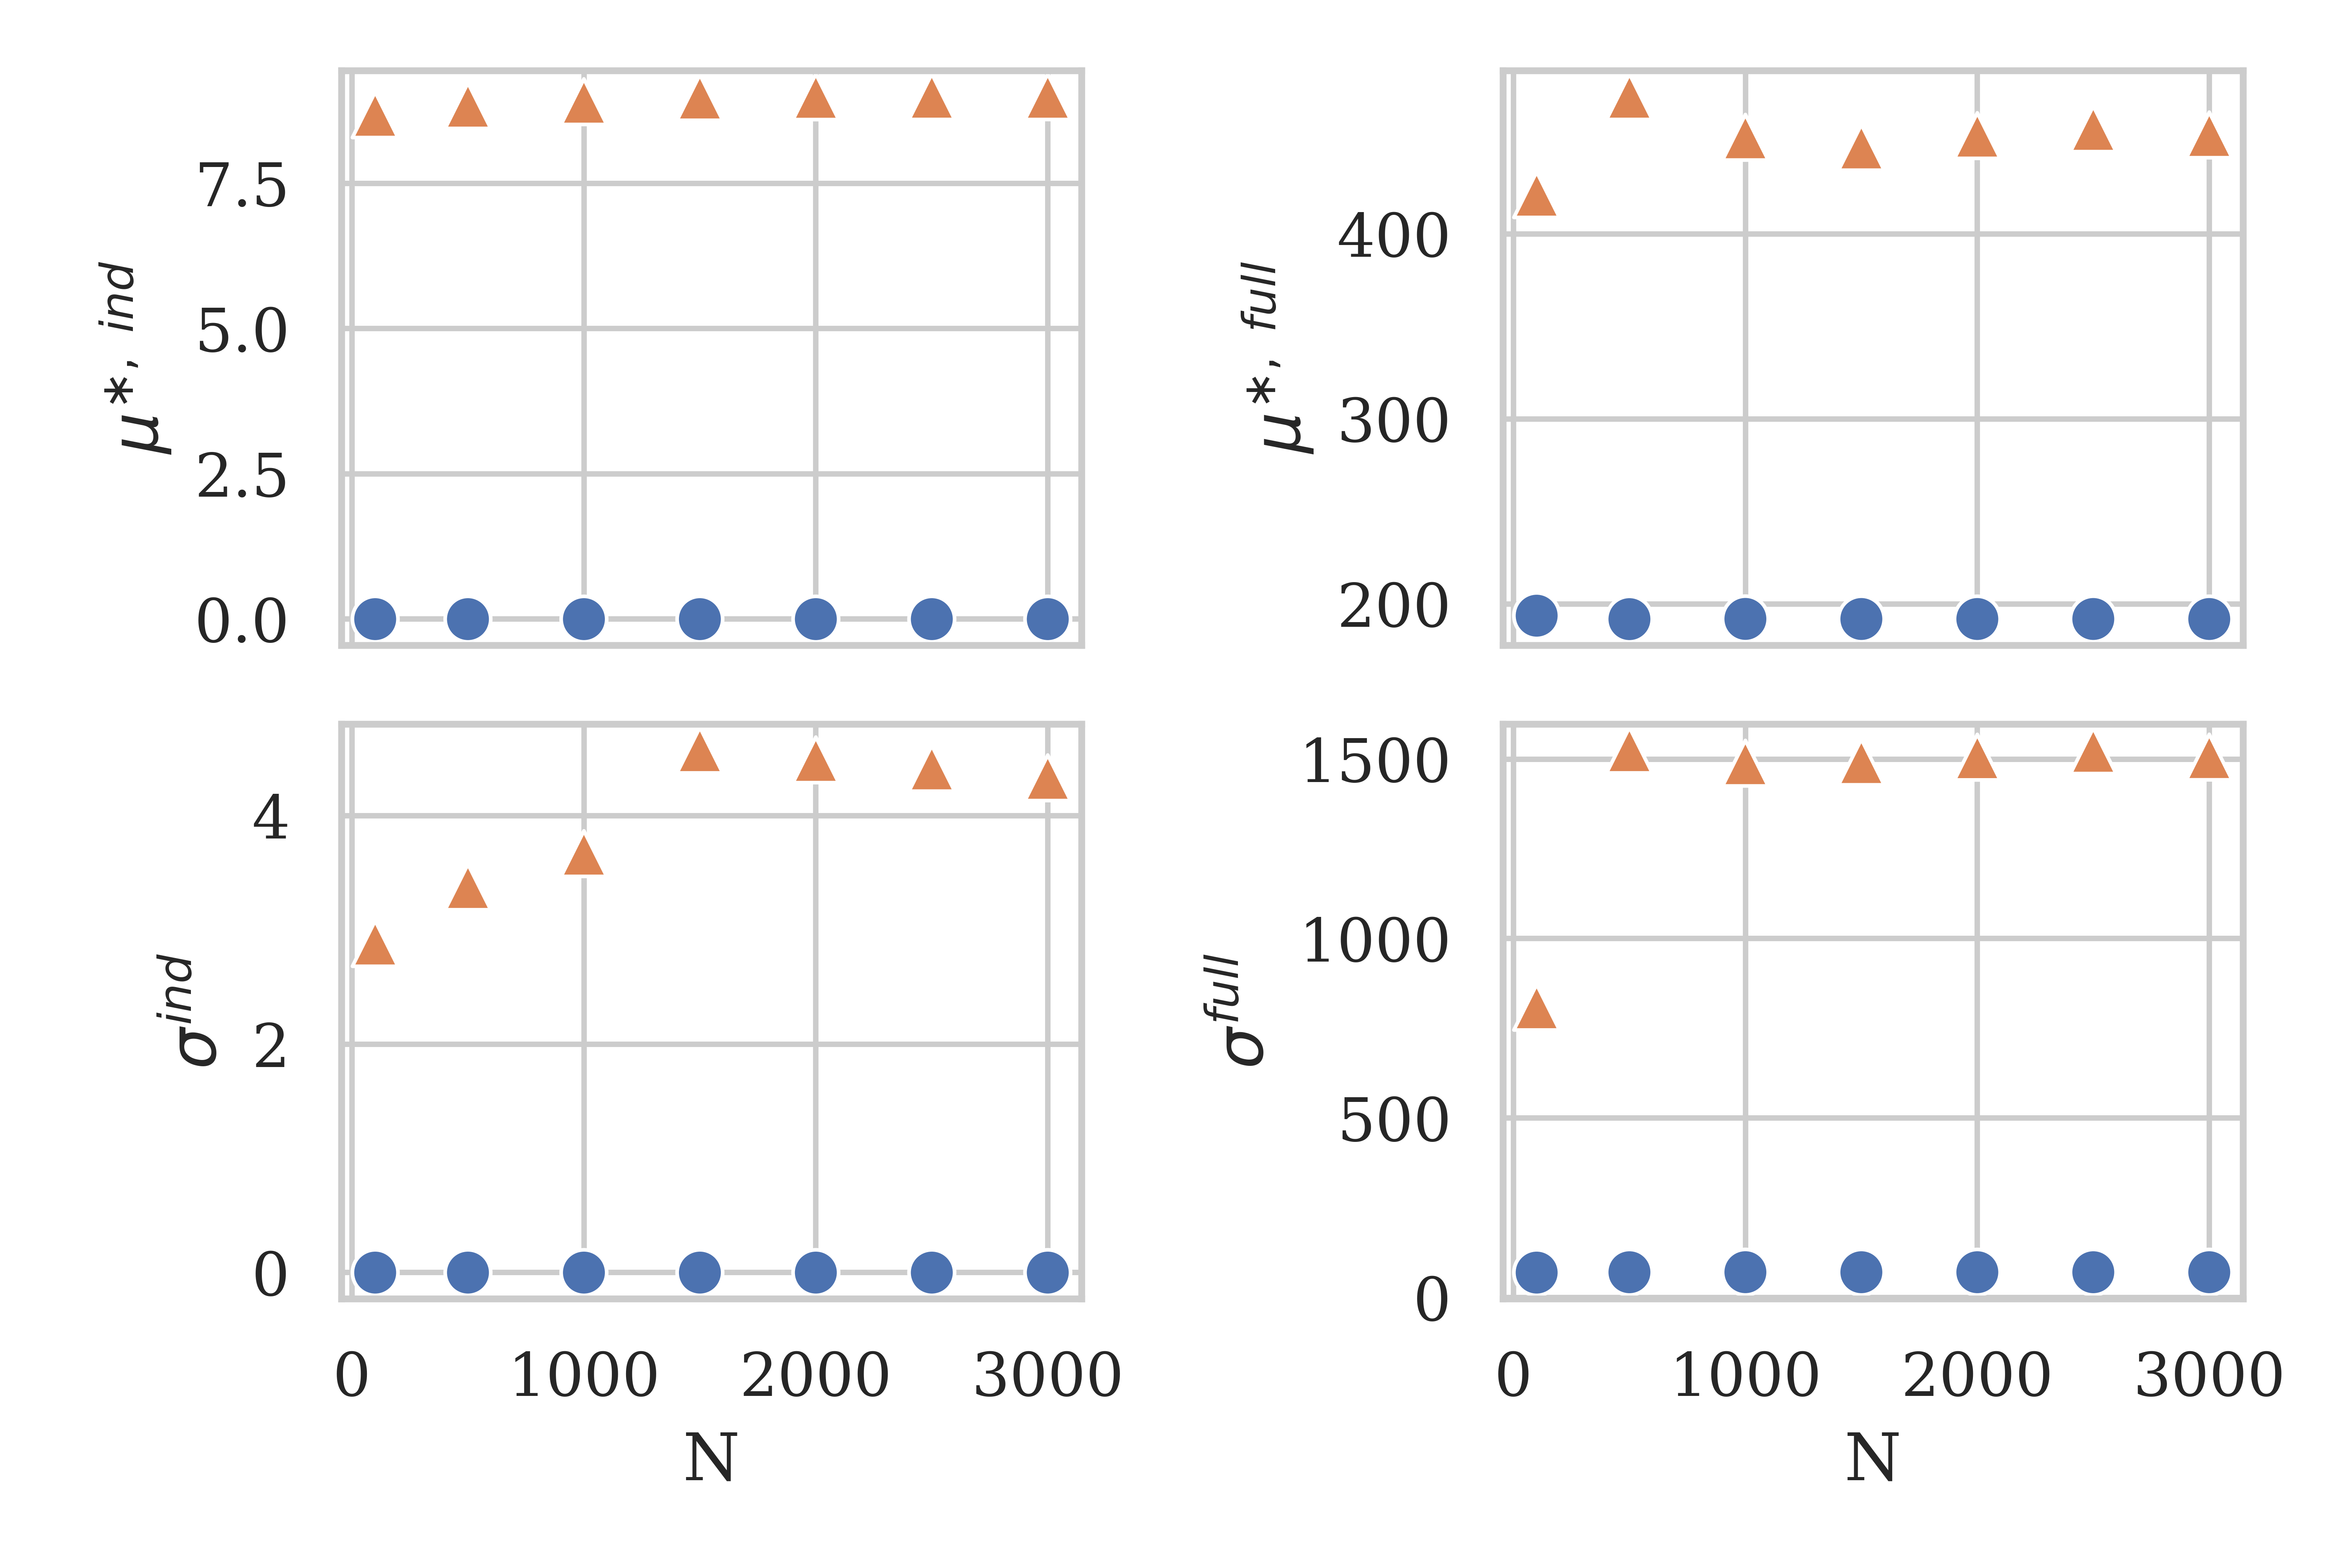
\includegraphics[scale=0.9]{../figures/morris_convergence.png}
\end{figure}

\begin{figure}[t]
	\caption{Uncertainty in Morris Indices - 100 Replicates}
    % \floatfoot{A note}
    \label{morris_replicates}
	\vspace*{-4mm}
	\centering
	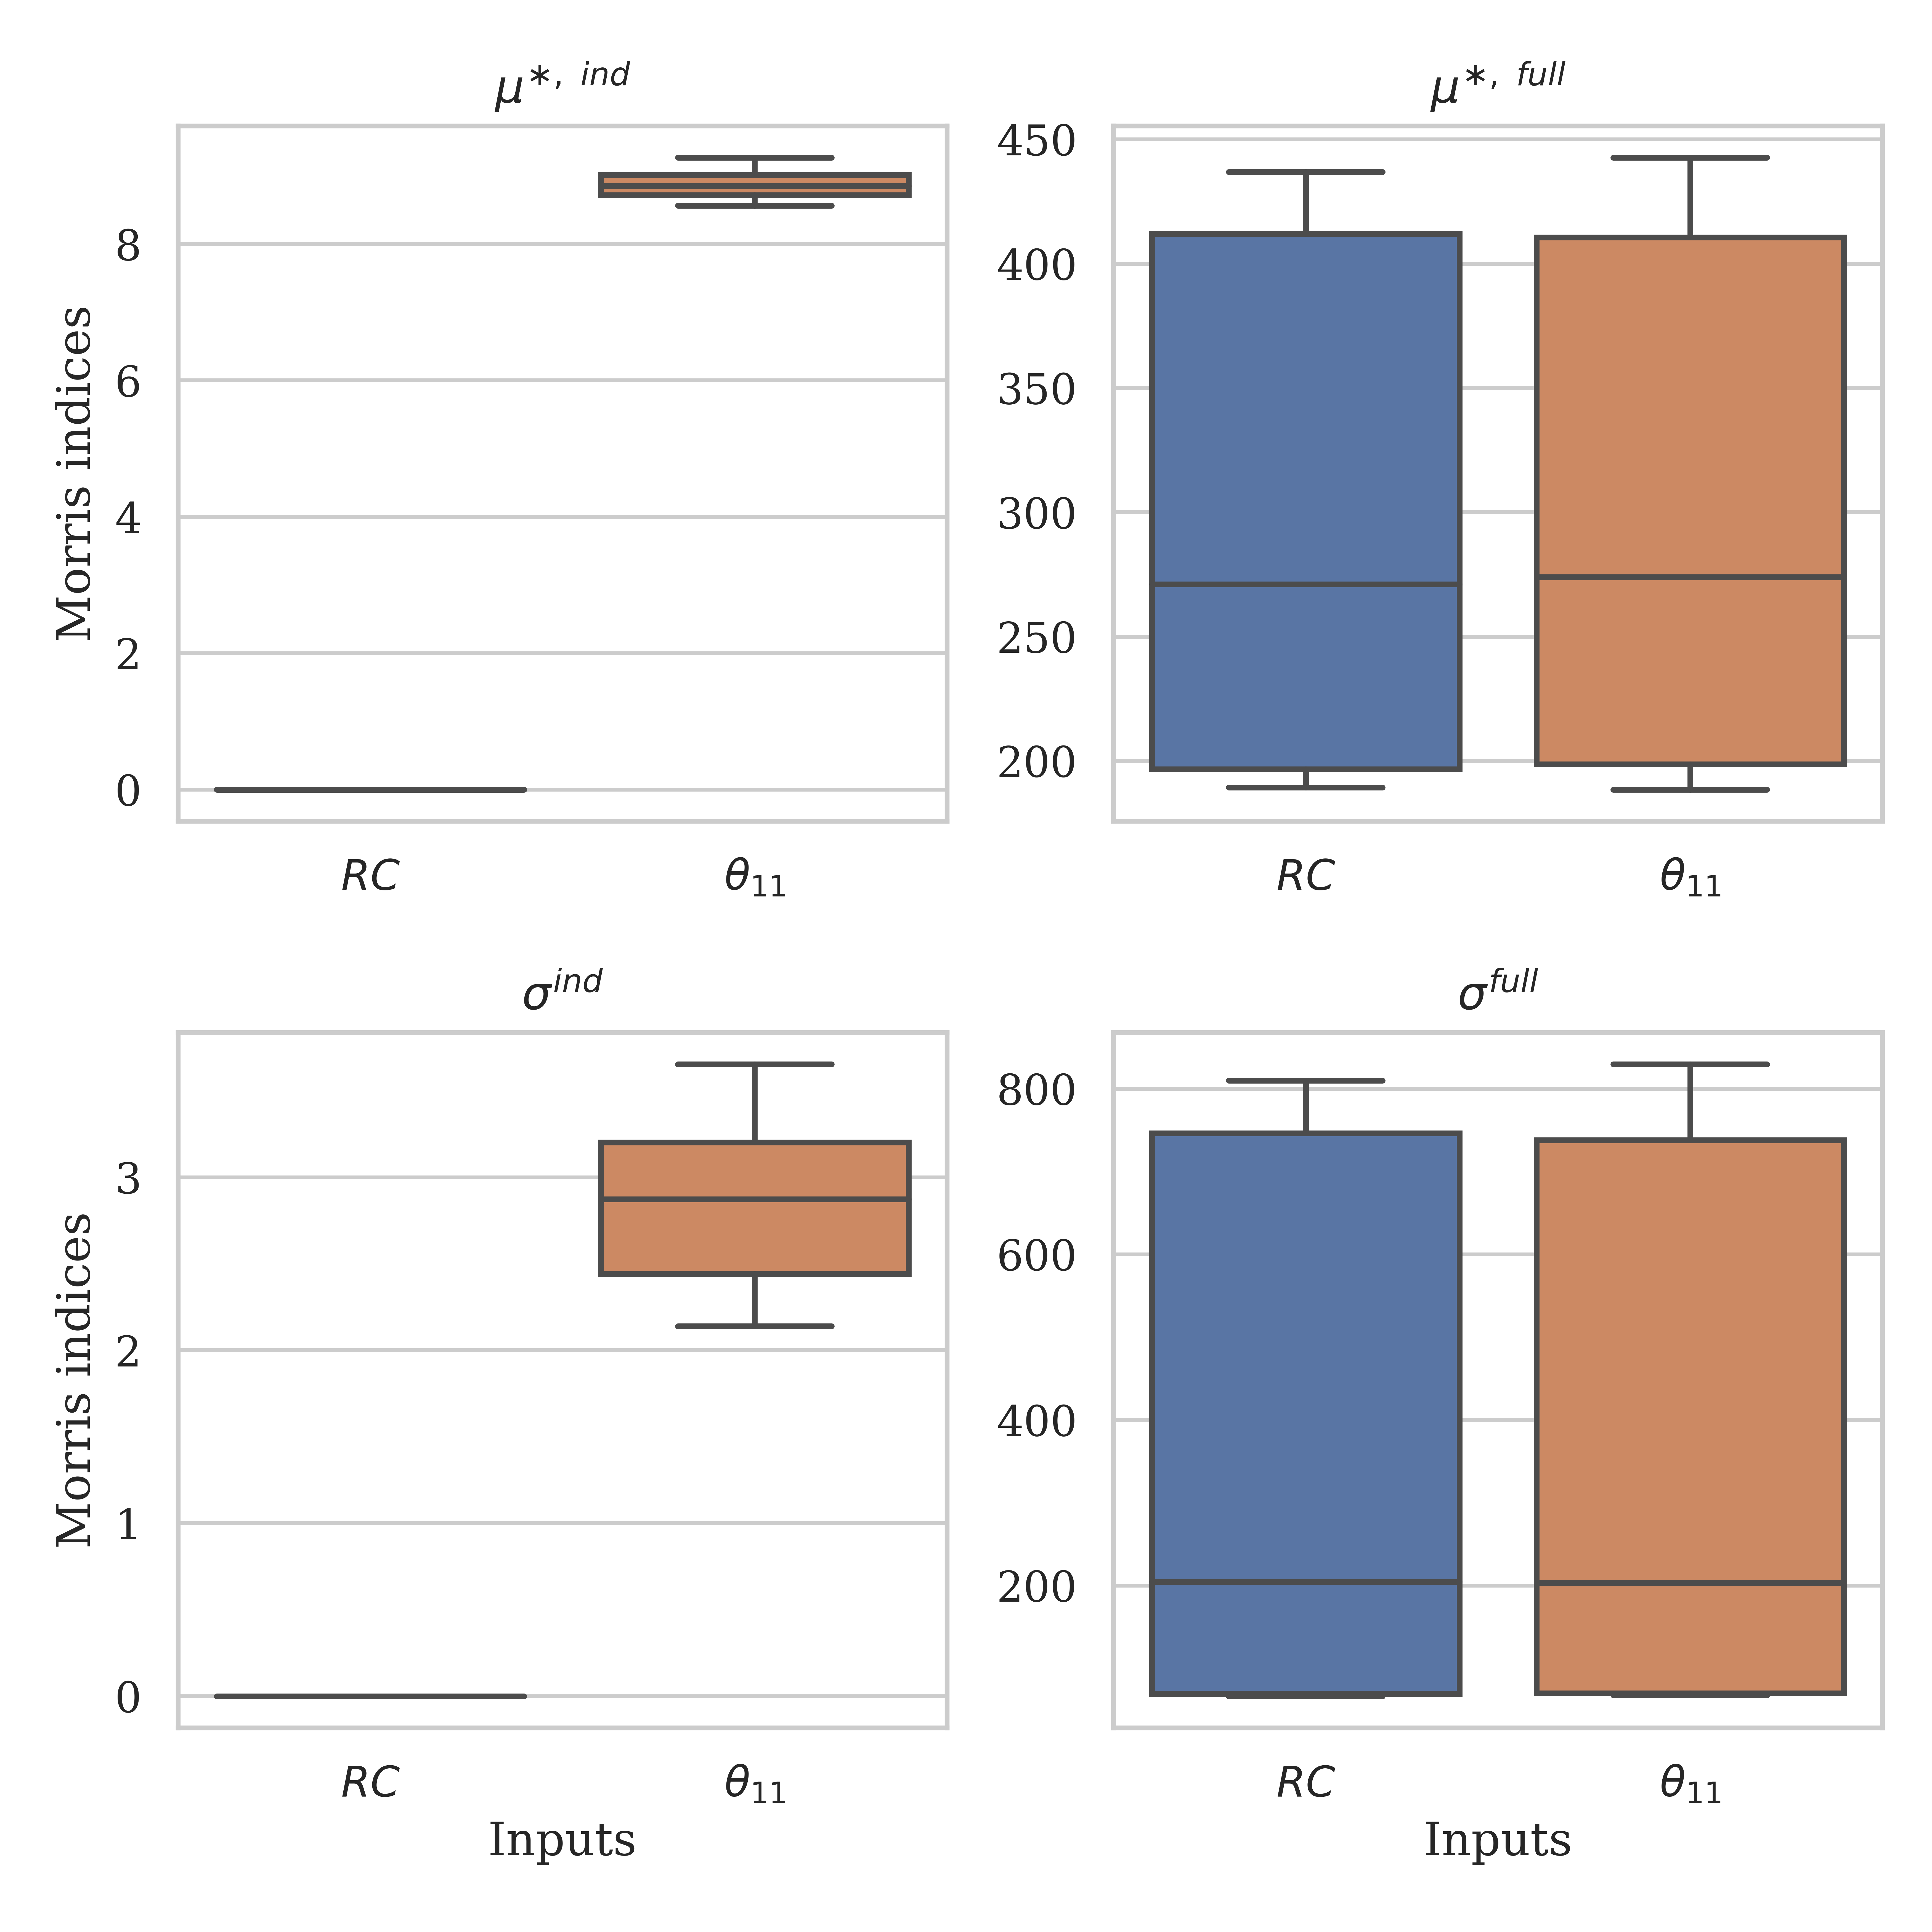
\includegraphics[scale=0.9]{../figures/boxplot_morris_replicates_100.png}
\end{figure}

% \begin{table}[!htbp]
%     \centering
%     \caption{Morris indices for different sample sizes}
%     \begin{threeparttable}
%     \centering

%     \begin{subtable}{2in}
%         % \centering
%         \caption{Sample size: 100}
%         \begin{tabular}{llrr}
\toprule
     &               &  $\mu^\ast$ &    $\sigma$ \\
Type & Input &             &             \\
\midrule
independent & $RC$ &    0.000000 &    0.000000 \\
     & $\theta_{11}$ &    8.680638 &    2.881537 \\
full & $RC$ &  193.619610 &   69.825364 \\
     & $\theta_{11}$ &  421.293224 &  808.934874 \\
\bottomrule
\end{tabular}

%     \end{subtable}

%     \centering
%     \begin{subtable}{2in}
%         % \centering
%         \caption{Sample size: 500}
%         \begin{tabular}{llrr}
\toprule
     &               &  $\mu^\ast$ &     $\sigma$ \\
Type & Input &             &              \\
\midrule
independent & $RC$ &    0.000000 &     0.000000 \\
     & $\theta_{11}$ &    8.837636 &     3.376486 \\
full & $RC$ &  191.756229 &    70.817395 \\
     & $\theta_{11}$ &  474.280390 &  1525.014109 \\
\bottomrule
\end{tabular}

%     \end{subtable}

%     \centering
%     \begin{subtable}[t]{2in}
%         \caption{Sample size: 1000}
%         \begin{tabular}{llrr}
\toprule
     &               &  $\mu^\ast$ &     $\sigma$ \\
Type & Input &             &              \\
\midrule
independent & $RC$ &    0.000000 &     0.000000 \\
     & $\theta_{11}$ &    8.906009 &     3.668524 \\
full & $RC$ &  191.873898 &    70.942862 \\
     & $\theta_{11}$ &  452.332338 &  1488.709509 \\
\bottomrule
\end{tabular}

%     \end{subtable}

%     \begin{tablenotes}
%     \small
%     \centering
%     \item This is where authors provide additional information about the data, including whatever notes are needed.
%     \end{tablenotes}

%     \end{threeparttable}
% \end{table}


\section{Comparing Shapley Effects and Morris Indices} \label{comparison}

In this section I want to connect and further discuss the results presented in \cref{shapley_rust_model}
and \cref{morris_rust_model}.

Interestingly, in the case of two inputs and when setting $N_I = 3$ as recommended
by \citet{SNS16}, the computational burden of both algorithms are parallel, when
considering $N$ and $N_O$. Then they differ by $N_V$ only, given that $N = N_O$. One drawback
of the Shapley effects as in the implementation of \citet{SNS16} is that one needs to
set more than one sample size. For applying the Morris method we need to specify only one sample size.
Both, Shapley effects and independent Morris indices, succeed in identifying the correct input
ranking, even for a relatively small sample size. The

\begin{table}
	\centering
	\caption{Accuracy of Morris Indices}
	\label{accuracy}
	\begin{threeparttable}
	\centering
	\begin{tabular}{lllr}
\toprule
               &     &         Type &  Accuracy \\
Measure & Comp. cost &              &           \\
\midrule
Shapley effects & 160 &            - &    100.00 \\
Morris indices & 162 &  independent &    100.00 \\
               & 162 &         full &     59.14 \\
               & 600 &  independent &    100.00 \\
               & 600 &         full &     34.00 \\
\bottomrule
\end{tabular}

	\begin{tablenotes}
	\small
	\item \textit{Notes:} Share of the correct input rankings for $100$ Morris indices based on $\mu^{\ast,\ full}$ and $\mu^{\ast,\ ind}$. As a benchmark, the accuracy of Shapley effects is presented. For Morris indices the accuracy for different sample sizes is reported.
	\end{tablenotes}
	\end{threeparttable}
\end{table}

With respect to the estimation precision, Morris indices are subject to larger uncertainty
than Shapley effects. As argued above, this estimation precision is not necessarily needed. If
the identification of uninfluential inputs is the purpose of sensitivity analysis, estimates need to be precise
only in the sense that they yield nonzero indices if an input is important and zero if they
are not influential. If input ranking is the goal, the situation is slightly different. The simulation
study presented in this paper with two inputs only may not be the right trial to investigate
this. In the case of the Rust model, a ranking based on the full Morris indices can be misleading, if the sample size is not large enough, since estimates are very volatile.

Since the estimation of Shapley effects is more costly and acknowledging that Morris
indices yield correct input rankings for the Rust model, one can resort to using the Morris
method for input importance ranking when interpreting the results with caution. For the Rust model, we can conclude that the influence of $RC$ is due to its dependence on $\theta_{11}$. Both, Shapley effects and Morris indices imply that more effort should be exerted into reducing uncertainty in $\theta_{11}$ if the derivation of more stable model output is the goal.

Further, Morris indices are informative about the model structure. Hence, one can not only successfully rank the inputs but also learn more about the model itself.

Since Shapley effects yield only one sensitivity index per input, they are easier to interpret than the four indices in the case of the Morris method.

My findings are broadly in line with the ones found in \citet{GM17} with the restriction that under small sample sizes full indices should not be used alone to derive the input ranking. The extension of the Morris method to dependent inputs is an important contribution.

\section{Conclusion} \label{conclusion}

% Was sind die Erkenntnisse, die Du gewonnen hast.

% Wie knüpfen die an vorherige Literatur an?

When independent indices are considered the extended Morris method proposed by \citet{GM17} successfully ranks model inputs according to their importance. This holds true even for small sample sizes. This is my main finding. It is only a valid substitute for Shapley effects if we apply sensitivity analysis for FF since full Morris indices successfully establish that both inputs of the Rust model are important, which is in line with the interpretation based on Shapley effects. My findings stress the importance of considering both, independent and full Morris indices, to identify an input as uninfluential. A conclusion based solely on the independent Morris indices can lead to Type II error in the case of the Rust model.

%It is therefore a valid substitute for Shapley effects if the purpose of sensitivity analysis is importance ranking or FF in the case of the Rust model.  My results are generally in line with the ones found in \citet{GM17}: this thesis adds one more piece of evidence in favour of the extended Morris method. This evidence hopefully encourages and facilitates the widespread application of sensitivity analysis in Economics. With the Morris method we have a easy to grasp and easy to implement sensitivity method, while performing well at low computational cost.

If FF is the purpose, none of the inputs of the Rust model can be fixed. Both, Shapley effects and Morris indices indicate this. This is a secondary finding of my analysis. The inherent uncertainty in the model inputs should not be ignored if one is to use the Rust model for policy making. We cannot assume that we knew neither of the two inputs with certainty. If uncertainty in implied annual demand is to be reduced, my investigation suggests that particular attention should be allocated to the slope parameter of the cost function $\theta_{11}$. Independent and full Morris indices show that the influence of the replacement costs, $RC$, on implied annual demand for bus engines is due to its dependence on the $\theta_{11}$ only.

% Lassen sich die Erkenntnisse verallgemeinern oder was sind Spezifika, die zu beachten sind?

Since \citet{GM17} do not provide formal arguments about the properties of Morris indices, it is not clear whether these findings generalise. Further research on the convergence properties of the extended Morris method, especially for full indices, is needed.

% Was sind offene Fragen für zukünftige Forschung.

\newpage
% \thispagestyle{plain} % suppress header.
\addcontentsline{toc}{section}{References}
\printbibliography[title={References}]

\end{document}